\documentclass[12pt]{article}
\usepackage{graphicx}
\usepackage{amssymb}

\begin{document}
%- https://www.tutorialspoint.com/discrete_mathematics/discrete_mathematics_sets.htm
\section*{Set Theory}
\Large
\begin{itemize}
\item[1.1] Introduction  
\item[1.2] Sets  
\item[1.3] Sub-sets  
\item[1.4] The order of sets: finite and infinite sets .
\item[1.5] Union and intersection of sets  
\item[1.6] Differences and complements  
\item[1.7] Venn diagrams  
\item[1.8] Logic analysis
\end{itemize}  
\newpage
German mathematician G. Cantor introduced the concept of sets. He had defined a set as a collection of definite and distinguishable objects selected by the means of certain rules or description.

Set theory forms the basis of several other fields of study like counting theory, relations, graph theory and finite state machines. In this chapter, we will cover the different aspects of Set Theory.


\subsection{Representation of a Set}
Sets can be represented in two ways −

Roster or Tabular Form
Set Builder Notation

%=====================================================%
Roster or Tabular Form
The set is represented by listing all the elements comprising it. The elements are enclosed within braces and separated by commas.

Example 1 − Set of vowels in English alphabet, A={a,e,i,o,u}A={a,e,i,o,u}
Example 2 − Set of odd numbers less than 10, B={1,3,5,7,9}B={1,3,5,7,9}
Set Builder Notation
The set is defined by specifying a property that elements of the set have in common. The set is described as A={x:p(x)}A={x:p(x)}
Example 1 − The set {a,e,i,o,u}{a,e,i,o,u} is written as −

\[A={x:x is a vowel in English alphabet}\]
%=====================================================%
\subsubsection*{Example 2} − The set ${1,3,5,7,9}$ is written as −

B={x:1\leqx<10 and (x%2)≠0}B={x:1\leqx<10 and (x%2)≠0}
If an element x is a member of any set S, it is denoted by x∈Sx∈S and if an element y is not a member of set S, it is denoted by y∉Sy∉S.

Example − If S={1,1.2,1.7,2},1∈SS={1,1.2,1.7,2},1∈S but 1.5∉S
%=====================================================%
\subsection{Some Important Sets}
\begin{itemize}
\item N − the set of all natural numbers = {1,2,3,4,.....}
\item Z − the set of all integers = {.....,−3,−2,−1,0,1,2,3,.....}
\item Z+ − the set of all positive integers
\item Q − the set of all rational numbers
\item R − the set of all real numbers
\item W − the set of all whole numbers
\end{itemize}

\subsection{Types of Sets}
Sets can be classified into many types. Some of which are finite, infinite, subset, universal, proper, singleton set, etc.

\subsection{Finite Set}
A set which contains a definite number of elements is called a finite set.

Example − S={x|x∈NS={x|x∈N and 70>x>50}70>x>50}
Infinite Set
A set which contains infinite number of elements is called an infinite set.

Example − S={x|x∈NS={x|x∈N and x>10}x>10}
Subset
A set X is a subset of set Y (Written as X⊆YX⊆Y) if every element of X is an element of set Y.

Example 1 − Let, X={1,2,3,4,5,6}X={1,2,3,4,5,6} and Y={1,2}Y={1,2}. Here set Y is a subset of set X as all the elements of set Y is in set X. Hence, we can write Y⊆XY⊆X.

Example 2 − Let, X={1,2,3}X={1,2,3} and Y={1,2,3}Y={1,2,3}. Here set Y is a subset (Not a proper subset) of set X as all the elements of set Y is in set X. Hence, we can write Y⊆XY⊆X.

\subsection{Proper Subset}
The term “proper subset” can be defined as “subset of but not equal to”. A Set X is a proper subset of set Y (Written as X⊂YX⊂Y) if every element of X is an element of set Y and |X|<|Y||X|<|Y|.

Example − Let, X={1,2,3,4,5,6}X={1,2,3,4,5,6} and Y={1,2}Y={1,2}. Here set Y⊂XY⊂X since all elements in YY are contained in XX too and XX has at least one element is more than set YY.

\subsection{Universal Set}
It is a collection of all elements in a particular context or application. All the sets in that context or application are essentially subsets of this universal set. Universal sets are represented as UU.

Example − We may define UU as the set of all animals on earth. In this case, set of all mammals is a subset of UU, set of all fishes is a subset of UU, set of all insects is a subset of UU, and so on.

Empty Set or Null Set
An empty set contains no elements. It is denoted by ∅∅. As the number of elements in an empty set is finite, empty set is a finite set. The cardinality of empty set or null set is zero.

Example − S={x|x∈NS={x|x∈N and 7<x<8}=∅7<x<8}=∅
Singleton Set or Unit Set
Singleton set or unit set contains only one element. A singleton set is denoted by {s}{s}.

Example − S={x|x∈N, 7<x<9}S={x|x∈N, 7<x<9} = {8}{8}
Equal Set
If two sets contain the same elements they are said to be equal.

Example − If A={1,2,6}A={1,2,6} and B={6,1,2}B={6,1,2}, they are equal as every element of set A is an element of set B and every element of set B is an element of set A.

Equivalent Set
If the cardinalities of two sets are same, they are called equivalent sets.

Example − If A={1,2,6}A={1,2,6} and B={16,17,22}B={16,17,22}, they are equivalent as cardinality of A is equal to the cardinality of B. i.e. |A|=|B|=3|A|=|B|=3
Overlapping Set
Two sets that have at least one common element are called overlapping sets.

In case of overlapping sets −

n(A∪B)=n(A)+n(B)−n(A∩B)n(A∪B)=n(A)+n(B)−n(A∩B)
n(A∪B)=n(A−B)+n(B−A)+n(A∩B)n(A∪B)=n(A−B)+n(B−A)+n(A∩B)
n(A)=n(A−B)+n(A∩B)n(A)=n(A−B)+n(A∩B)
n(B)=n(B−A)+n(A∩B)n(B)=n(B−A)+n(A∩B)
Example − Let, A={1,2,6}A={1,2,6} and B={6,12,42}B={6,12,42}. There is a common element ‘6’, hence these sets are overlapping sets.

Disjoint Set
Two sets A and B are called disjoint sets if they do not have even one element in common. Therefore, disjoint sets have the following properties −

n(A∩B)=∅n(A∩B)=∅
n(A∪B)=n(A)+n(B)n(A∪B)=n(A)+n(B)
Example − Let, A={1,2,6}A={1,2,6} and B={7,9,14}B={7,9,14}, there is not a single common element, hence these sets are overlapping sets.

Venn Diagrams
Venn diagram, invented in 1880 by John Venn, is a schematic diagram that shows all possible logical relations between different mathematical sets.

Examples

Venn Diagram
Set Operations
Set Operations include Set Union, Set Intersection, Set Difference, Complement of Set, and Cartesian Product.

Set Union
The union of sets A and B (denoted by A∪BA∪B) is the set of elements which are in A, in B, or in both A and B. Hence, A∪B={x|x∈A OR x∈B}A∪B={x|x∈A OR x∈B}.

Example − If A={10,11,12,13}A={10,11,12,13} and B = {13,14,15}{13,14,15}, then A∪B={10,11,12,13,14,15}A∪B={10,11,12,13,14,15}. (The common element occurs only once)

Set Union
Set Intersection
The intersection of sets A and B (denoted by A∩BA∩B) is the set of elements which are in both A and B. Hence, A∩B={x|x∈A AND x∈B}A∩B={x|x∈A AND x∈B}.

Example − If A={11,12,13}A={11,12,13} and B={13,14,15}B={13,14,15}, then A∩B={13}A∩B={13}.

Set Intersection
Set Difference/ Relative Complement
The set difference of sets A and B (denoted by A–BA–B) is the set of elements which are only in A but not in B. Hence, A−B={x|x∈A AND x∉B}A−B={x|x∈A AND x∉B}.

Example − If A={10,11,12,13}A={10,11,12,13} and B={13,14,15}B={13,14,15}, then (A−B)={10,11,12}(A−B)={10,11,12} and (B−A)={14,15}(B−A)={14,15}. Here, we can see (A−B)≠(B−A)(A−B)≠(B−A)Set Difference
Complement of a Set
The complement of a set A (denoted by A′A′) is the set of elements which are not in set A. Hence, A′={x|x∉A}A′={x|x∉A}.

More specifically, A′=(U−A)A′=(U−A) where UU is a universal set which contains all objects.

Example − If A={x|x belongstosetofoddintegers}A={x|x belongstosetofoddintegers} then A′={y|y doesnotbelongtosetofoddintegers}A′={y|y doesnotbelongtosetofoddintegers}Complement Set


Bell Numbers
Bell numbers give the count of the number of ways to partition a set. They are denoted by BnBn where n is the cardinality of the set.

Example −

Let S={1,2,3}S={1,2,3}, n=|S|=3n=|S|=3
The alternate partitions are −

1. ∅,{1,2,3}∅,{1,2,3}

2. {1},{2,3}{1},{2,3}

3. {1,2},{3}{1,2},{3}

4. {1,3},{2}{1,3},{2}

5. {1},{2},{3}{1},{2},{3}

Hence B3=5
%-----------------------------------------------------%
\newpage
\subsection*{Union and intersection of sets}

\begin{itemize}
\item The \textbf{union} of two sets A and B is a set containing all the elements in
either A or B (or both)
i.e. 
\[A \cup B = {x / x \in A \mbox{ or } x \in B}.\]
\item The \textbf{intersection} of two sets A and B is a set containing all the elements
that are both in A and B
i.e. 
\[A \cap B = {x / x \in A \mbox{ and }x \in B}\].

\item If sets A and B have no elements in common, i.e. $A \cap B = \emptyset$,then A and B
are termed \textbf{disjoint sets}.
\end{itemize}
\newpage
\subsection*{Subsets}

\begin{itemize}
\item Proper Subsets
\end{itemize}
\subsection*{The Power Set}

\newpage
\subsection*{Venn Diagrams}
\begin{figure}
\centering
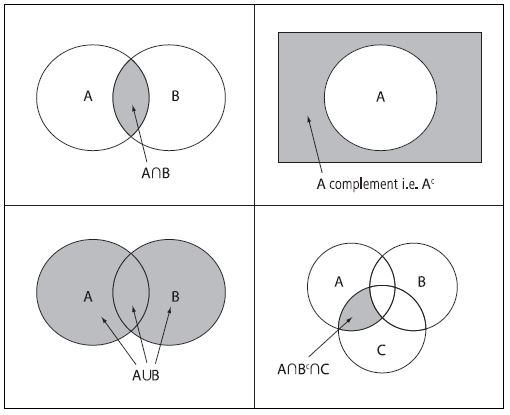
\includegraphics[width=0.7\linewidth]{venndiagram}

\end{figure}

\end{document}


